\subsection{Gaussian/Uniform Noise}
To analyze the third image provided, a histogram of both the whole image and the uniform coloured area was computed.
This is seen in figure \ref{fig:hist_pre_im03} and \ref{fig:hist_uni_im03}.


\begin{figure}[H]
\centering
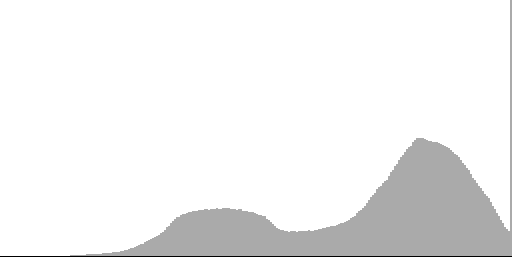
\includegraphics[width= \histogramWidth]{../code/images/histogram_full_pre_03}
\caption{Histogram of the full image 3.}
\label{fig:hist_pre_im03}
\end{figure}

The histogram in figure \ref{fig:hist_pre_im03} shows that the image contains a large amount of light colors.
This should be corrected for to improve the visual appearance of the image.
Furthermore, when considering figure \ref{fig:hist_uni_im03}, then the image also contains a mix of Gaussian and uniform noise.
Uniform because of the flat top of the noise distribution in figure \ref{fig:hist_uni_im03} and Gaussian since the bell-shape-like curves on the two sides.


\begin{figure}[H]
\centering
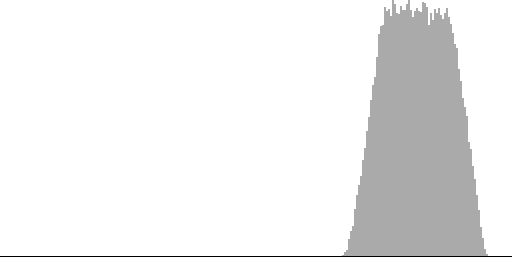
\includegraphics[width= \histogramWidth]{../code/images/histogram_uniform_03}
\caption{Histogram of the uniform area of image 3.}
\label{fig:hist_uni_im03}
\end{figure}


In order to fix both problems in the image, a set of different approaches can be taken.
The intensity of the image can be improved by either using a histogram-equalization or an intensity correction.
The advantage of the former is that this would also improve the contrast of the image whereas the latter only adjusts the brightness.

When a visual inspection of the two approaches is made, it is clear that the image improves the most with the intensity correction.
This is because the histogram-equalization also affects the noise present in the image and spreads it out in a broader color range, making the damage look considerably more sever.
This is also the case when applying the histogram-equalization to the image after reducing the noise, with the method proposed for noise reduction below.
The magnitude of intensity correction was found by visual inspection to be -25 when the image has a depth of eight bits.


In order to reduce the Gaussian/uniform noise present in the image a mean filter is considered.
This is because it is additive noise and mean filters work well on those.

For this image the three mean filters arithmetic-, geometric- and harmonic mean filters were considered.
With visual inspection it is clear that the arithmetic filter performs considerably worse than the two other filters, geometric and harmonic.
When it comes to telling if the geometric or harmonic filters apart, it is not directly visible to the human eye which of the two resulting images are the best.
It was however found that a filter size of five gives a descend noise reduction, without blurring the information too much.

In order to compare the results from the geometric and harmonic images, the difference between the two in the complex area of the image is shown in figure \ref{fig:diff_harVSgeo_im03}.



\begin{figure}[H]
\centering
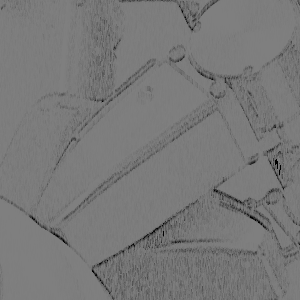
\includegraphics[width= \cutOutWidth]{../code/images/image_harVSgeo_complex_03}
\caption{Image difference between harmonic and geometric mean filtering in the complex area of image 3.}
\label{fig:diff_harVSgeo_im03}
\end{figure}


In figure \ref{fig:diff_harVSgeo_im03}, the amplified difference between the two images is plotted.
This was accomplished using equation \ref{eq:img_diff_harVSgeo}, where $I_{diff}$, $I_{har}$ and $I_{geo}$ is the intensity of the difference image, harmonic mean filtered and geometric mean filtered image respectively and $A$ is the scalar the difference is amplified with.

% \begin{equation}
% I_{diff} = \left( I_{har} - I_{geo} \right) * A + 127
% \label{eq:img_diff_harVSgeo}
% \end{equation}

For this image a $A$ of five was used.
Figure \ref{fig:diff_harVSgeo_im03} displays in dark/black the pixels of which the geometric mean filter gave the highest intensity, white for which it was the harmonic and grey for the values which are approximately equal.

On figure \ref{fig:diff_harVSgeo_im03} the edges are indicated in black.
Since it is wanted to have the clearest edges as possible on the image, the lowest possible intensity is wanted.
It can from this be concluded that the harmonic filter preserves the edges better than the geometric filter for this image.
Therefore it was decided to use the harmonic mean filter to restore the image.


\begin{figure}[H]
\centering
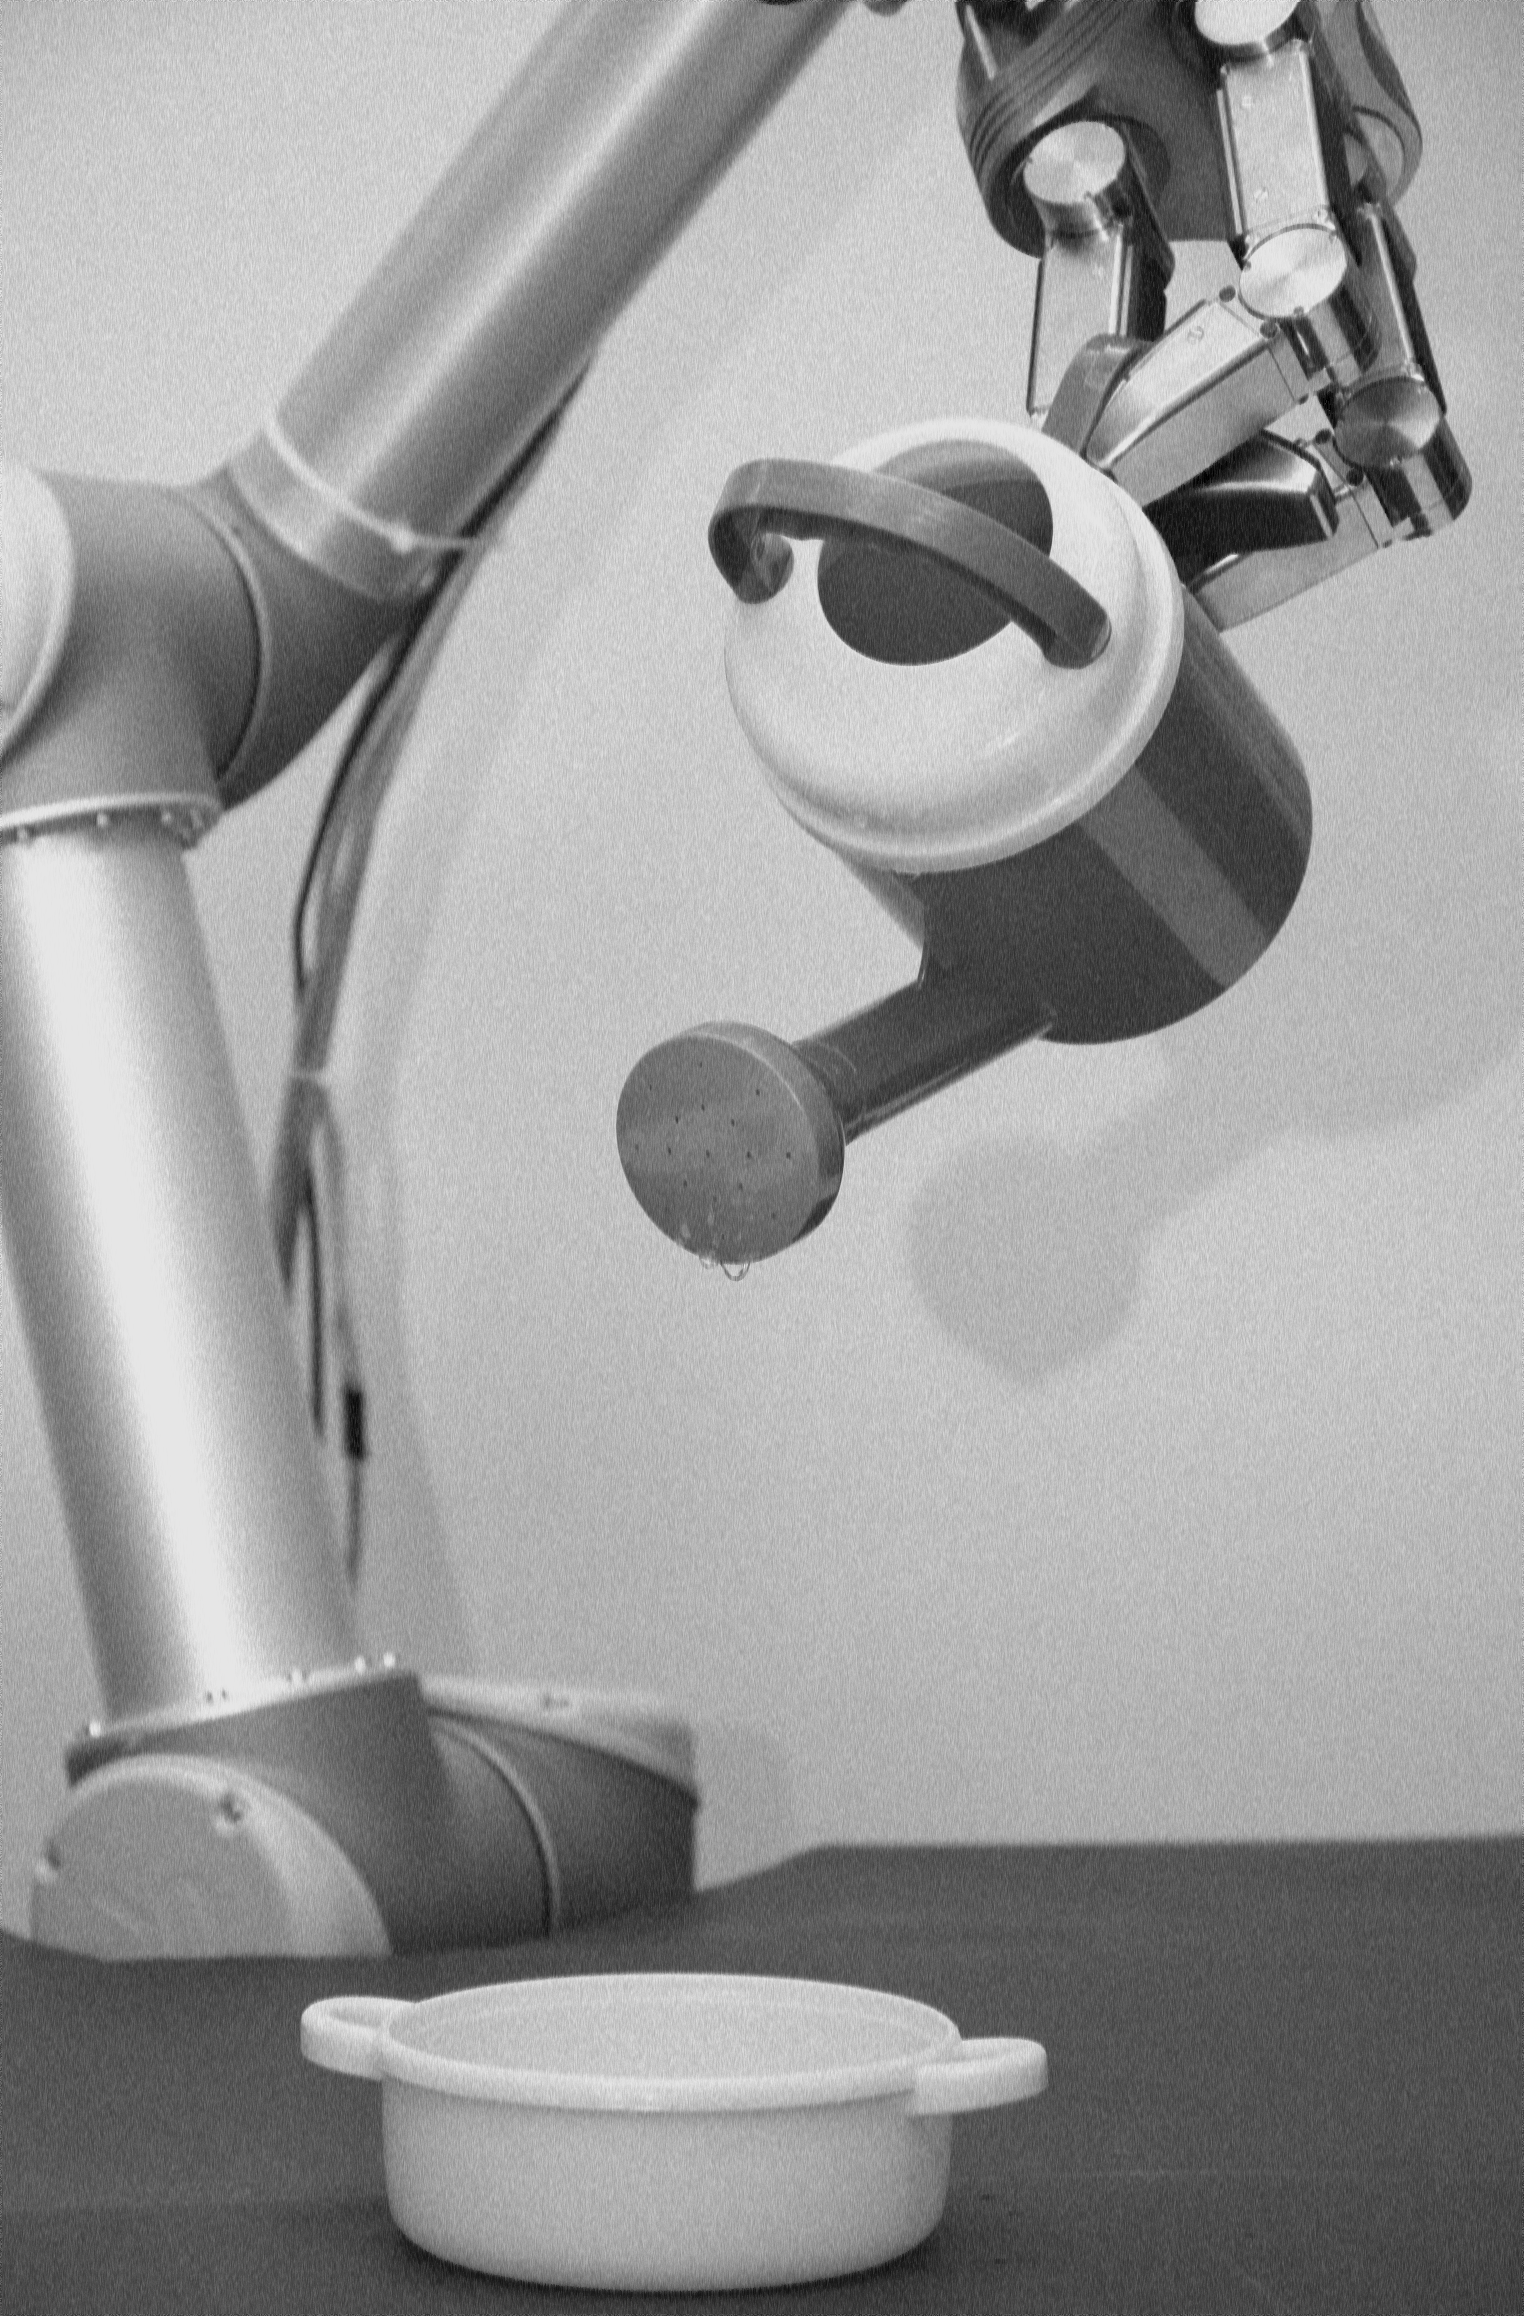
\includegraphics[width= \fullImageWidth]{../code/images/image_harmonic_03}
\caption{Resulting image after filtering using the harmonic mean and kernel size of five on image 3 with intensity correction.}
\label{fig:img_result_im03}
\end{figure}


The resulting picture using both the intensity adjustment and harmonic filter is seen in figure \ref{fig:img_result_im03}.
%From here both the histogram of the full image and the uniform area of the image is plotted resulting in figure \ref{fig:hist_post_im03} and \ref{fig:hist_uni_geo_im03} respectively.
The histogram of the uniform area of the resulting image is plotted in figure  \ref{fig:hist_uni_har_im03}.


\begin{figure}[H]
\centering
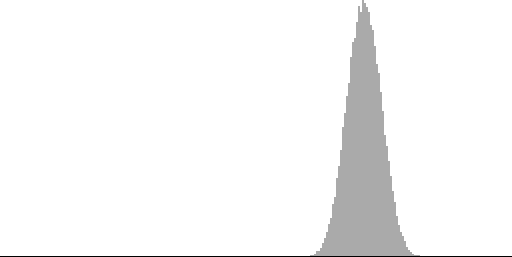
\includegraphics[width= \fullImageWidth]{../code/images/histogram_uniform_harmonic_03}
\caption{Histogram of the uniform area of image 3 after applying harmonic mean filter with kernel size of five and intensity adjustment.}
\label{fig:hist_uni_har_im03}
\end{figure}


It can from figure \ref{fig:hist_uni_har_im03} be seen that the process correctly shifts the mean to the left, by the amount chosen for the intensity correction, and then filters the image into a narrower normal distribution than that seen in figure \ref{fig:hist_uni_im03}, yielding a visually better image than initially.

The resulting process is thus:
\begin{itemize}
 \item Intensity shift of -25.
 \item Harmonic Mean filter, kernel size of 5x5.
\end{itemize}

%\begin{figure}[H]
%\centering
%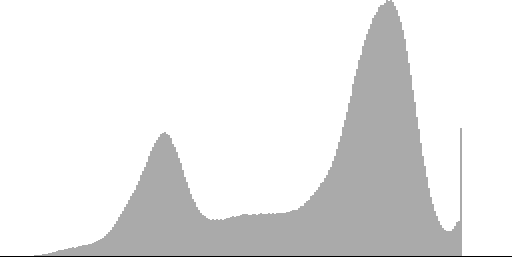
\includegraphics[width= 0.9 \linewidth]{../code/images/histogram_full_post_03}
%\caption{Histogram of the full resulting image 3.}
%\label{fig:hist_post_im03}
%\end{figure}
